\section{Evaluation in PlanetLab}
\label{sec:deploy}

In this section we evaluate \dtrack{} with local remapping in PlanetLab.
We are limited to PlanetLab as other measurements platforms such
as RIPE Atlas do not support custom measurement tools.  We deployed a
modified version of \dtrack{} in 95 PlanetLab nodes and collected
measurements for one week starting April 19th, 2014.  Our modified
\dtrack{} runs local remapping and complete remapping whenever it
detects a path change.  As in the data set used in the previous
sections, each PlanetLab node has a detection budget of 8 probes per
second and monitors 1,000 destinations chosen randomly from a list of
34,820 reachable destinations in the Internet.  We observed 1,228,559
path changes.  The observed paths traverse 6291 ASes and 96\% of the
ASes with more than 50 customers~\cite{luckie13asrel}.

\figstr~\ref{fig:deploy.savings} shows probing cost savings when using
local remapping instead of complete remapping in the real deployment.
Comparing with \figstr~\ref{fig:sim.savings.cmp}, the average cost
savings in the real deployment are qualitatively similar to the results
we obtained via simulation (solid lines).  Local remapping reduces
probing cost by more than half for 92\% of path changes in the real
deployment, and reduces overall probing cost by 75\%.  Two factors may
explain why probing savings are slightly higher than in the trace-driven
simulations.  First, the set of paths and the monitoring period are
different.  Second, \dtrack{} targets more detection probes at the last
radii of paths, whereas in the simulations we distribute detection
probes uniformly over all radii.

% 79\% of path changes have divergence hop in the second half of paths

% IMPROVEMENTS:
%
% log detection radius so we can check whether it has an impact on
% savings and accuracy
%
% choose remaprt paths instead of paris traceroute's so we live with
% temporary remapping errors

% \begin{figure}
% \begin{center}
% 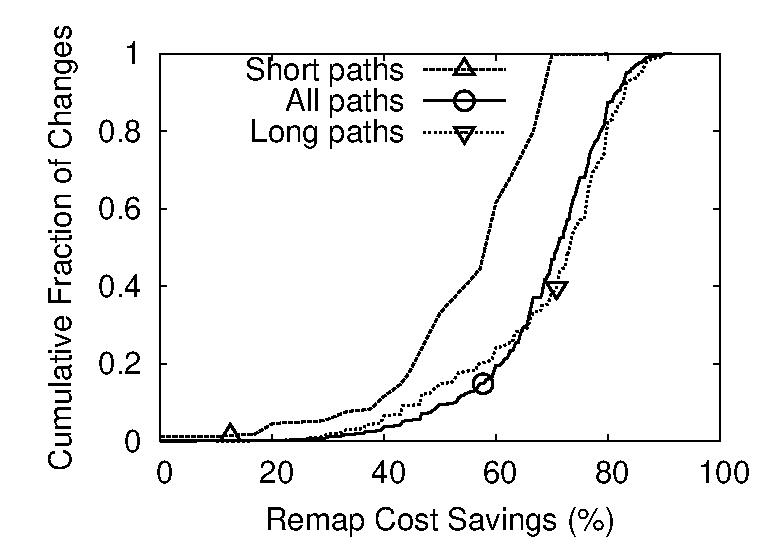
\includegraphics[width=0.8\columnwidth]{figs/deploysavings.eps}
% \caption{Remap cost savings with \rmprt{} in real scenarios.}
% \label{fig:deploy.savings}
% \end{center}
% \end{figure}

% Remap cost savings for short and long routes are more similar to the
% average savings in the real deployment than in the simulations.  In
% other words, the dashed lines in \figstr~\ref{fig:deploy.savings} are
% closer to the solid line than in \figstr~\ref{fig:sim.savings.cmp}.  We
% attribute this change to two factors: (i) the smaller number of observed
% changes may limit the variety of observed changes and (ii) differences
% in the set of monitored paths.\ed{Check text when we get the new
% results.}

\figstr~\ref{fig:deploy.latency} shows the distribution of remapping
latency for local remapping and complete remapping for all changes in
our data sets.  We study latency because local remapping
measures hops sequentially: the next hop to measure is computed based on
the observation at the last measured hop.  Traceroute, however, could
parallelize probing of different hops.  As most path changes require
measuring only a few hops (\figstr~\ref{fig:sim.abs.cmp}), remapping
latency is generally less than 5 seconds.  Complete remapping's
remapping latency is significantly higher, as Paris traceroute's MDA
measures hops sequentially.  We note remapping latency is heavily
affected by implementation choices, but these results show that local
remapping latency is acceptable for use in real systems.  We also note
that \dtrack{} can execute local remapping simultaneously on different
paths if more than one path change is detected in a short time interval.

% \figstr~\ref{fig:deploy.latency} shows the $25^\mathrm{th}$, the
% $50^\mathrm{th}$, and the $75^\mathrm{th}$ percentiles of \rmprt{}'s
% remap latency as a function of the number of hops probed during the
% remapping process.  We studied the remap latency because \rmprt{} probes
% hops sequentially: the next hop to probe is computed based on the result
% of the last probed hop.  Paris traceroute, however, could parallelize
% probing of different hops (but the classic implementation does not).  As
% most \rmprt{} remaps require probing only a few hops
% (\figstr~\ref{fig:sim.abs.cmp}), remapping latency is generally less
% than 5 seconds.  \figstr~\ref{fig:deploy.latency.ptr} shows the
% $25^\mathrm{th}$, the $50^\mathrm{th}$, and the $75^\mathrm{th}$
% percentiles of Paris traceroute's remapping latency in the real
% deployment.  Our objective is not to compare \rmprt{}'s and Paris
% traceroute's remapping latency, as latency is heavily affected by
% implementation choices.  Our objective is to show that \rmprt{}'s
% remapping latency is acceptable for use in real systems.  We also note
% that a topology mapping system like \dtrack{} can execute \rmprt{}
% simultaneously on different paths if more than one path change is
% detected in a short time interval.

% \begin{figure}
% \begin{center}
% 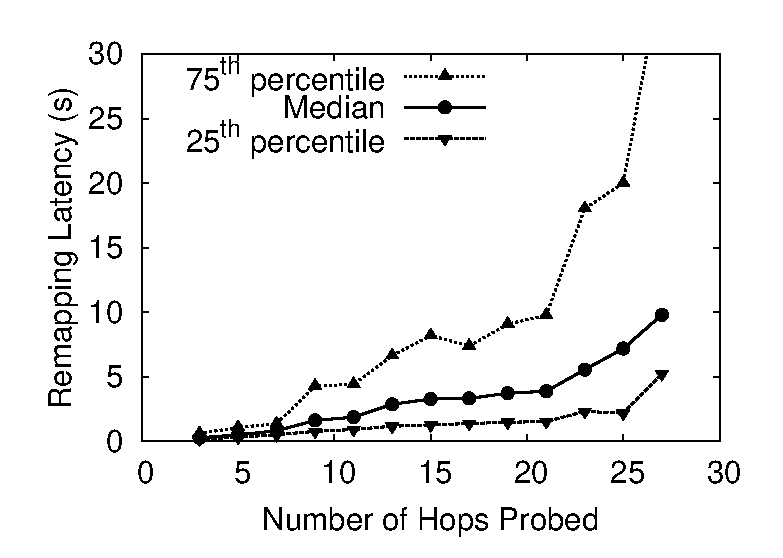
\includegraphics[width=0.8\columnwidth]{figs/latency.eps}
% \caption{RemapRoute remap latency in the real deployment.}
% \label{fig:deploy.latency}
% \end{center}
% \end{figure}

% \begin{figure}
% \begin{center}
% 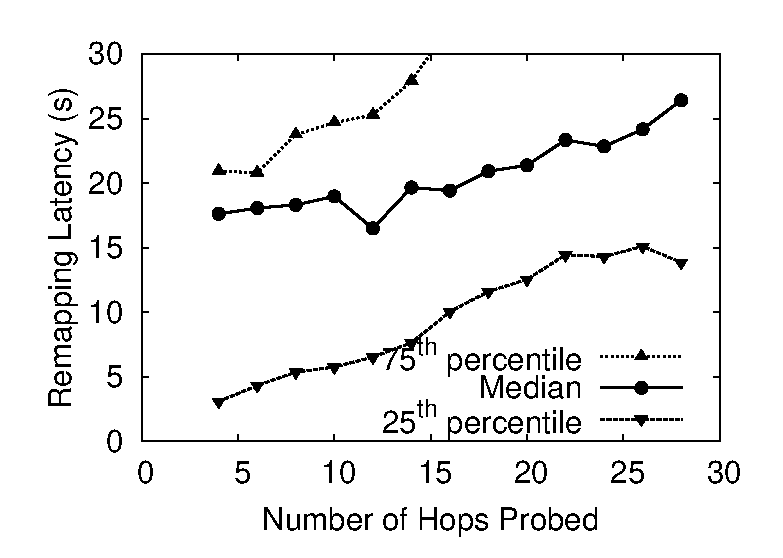
\includegraphics[width=0.8\columnwidth]{figs/ptrlatency.eps}
% \caption{Paris traceroute remap latency in the real deployment.}
% \label{fig:deploy.latency.ptr}
% \end{center}
% \end{figure}

Finally, we also evaluate accuracy, or whether routes measured with
local remapping are equivalent to those measured with complete remapping.
For each observed change in the real deployment, we compare the new
route measured with local remapping and the new route measured with
complete remapping.  We find that local remapping discovers the same
route as complete remapping for 92\% of path changes.  Errors occur
mainly in two cases. In 4.2\% of path changes, local remapping fails to
detect and remap multiple $\LCZ$s. These cases are a limitation local
remapping that results in temporary inconsistencies in the data set
(\secstr~\ref{sec:remap.errors}). In 3.4\% of path changes, local
remapping discovers different branches under load balancing than
complete remapping. The identification of routers that perform load
balancing is probabilistic~\cite{veitch09balancer}.  For example, Paris
traceroute's MDA identifies all interfaces in a path with 95\%
confidence.  Estimation errors are inevitable and cause inference of
different branches regardless of remapping method.  Another cause for
different measurements are path changes that happen during remapping.

% 0.2\% reorderings

In summary, local remapping is almost as accurate as complete remapping,
significantly reduces probing cost, and finishes quickly.
